% !TEX root = ../main.tex
\section{Introduction}
\label{introduction}

An often cited statistic is that data scientists spend 80\% of their time finding, preparing, integrating and cleaning data sets. The remaining 20\% is spent doing useful work (i.e. the desired analysis tasks). In fact, 80\% may be a lower bound; for example one data officer (Mark Schreiber of Merck) estimates his data scientists spend 98\% of their time on ``mung work'' and only one hour per week on ``useful work''. 

In this paper, we present \dcv, a system we are building at MIT, QCRI, Waterloo, and TU Berlin, whose main purpose is to decrease the ``mung work factor'', by helping data scientists:

\vspace{.5em}
%\begin{itemize} \\

\noindent i) perform data discovery; i.e. quickly find data of interest from large numbers of tables, 

\vspace{.5em}

\noindent ii) perform data stitching; i.e. find ways to connect up data sets of interest, 

\vspace{.5em}

\noindent iii) execute queries to fetch desired data from disparate data stores, 

\vspace{.5em}

\noindent iv) clean the required data, as it is often citied that 20\% of a typical data source is incorrect or missing,

\vspace{.5em}

\noindent v) perform these tasks iteratively using a workflow system, since data scientists often iterate though these steps in different orders. 

\vspace{.5em}
%\end{itemize}

\dcv focuses on structured data, which is represented as a collection of (sparse or dense) tables.  We assume that text has been parsed in advance into a structured representation, and that file data can be “tableized” by an adaptor.

\dcv consists of a collection of modules with a workflow scheduling system, as noted in the architecture diagram of Figure 1. We elaborate on each of modules in the remainder of this section, using Merck as an example. 



\begin{figure}[!t]
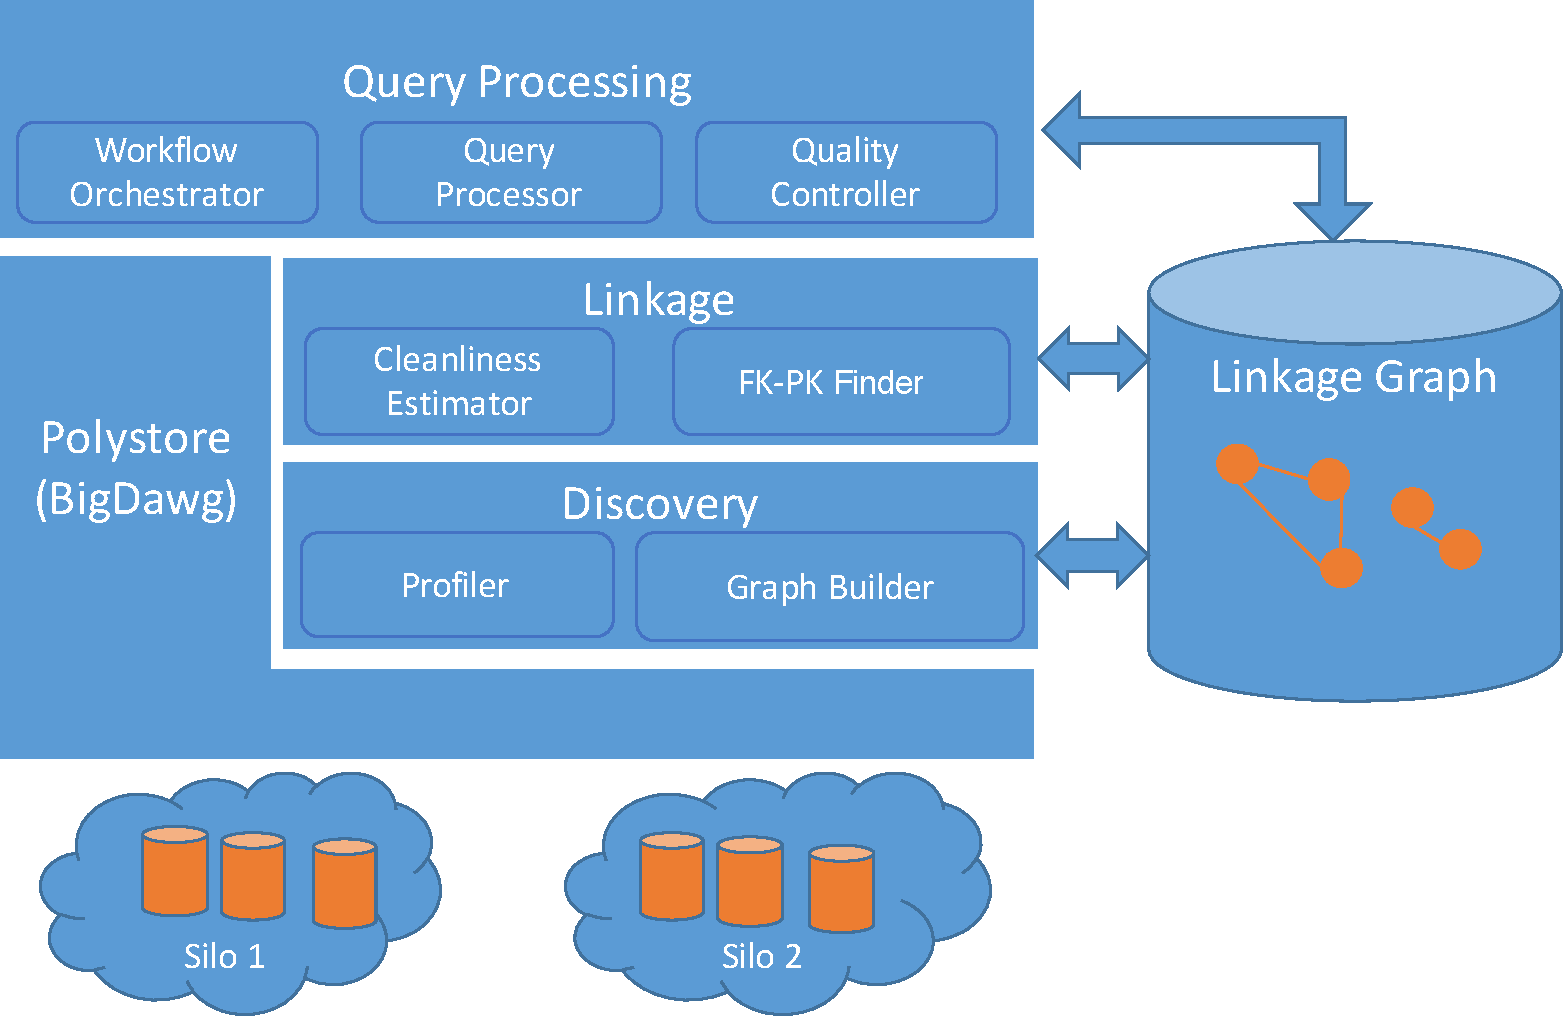
\includegraphics[width=3.5in]{arch3.pdf}
\caption{\dcv Architecture}
\label{fig:arch}
\end{figure}


\stitle{[Discovery]} A data scientist at Merck has a hypothesis, for example, {\it the drug Ritalin causes brain cancer in rats weighing more than 300 grams}.  His first job is to identify relevant data sets, both inside and outside of Merck, that might contribute to testing this hypothesis. Inside the company alone, Merck has approximately 4,000 Oracle databases and countless other repositories. The discovery component in \dcv, discussed in Section~\ref{sec:discovery}, assists the scientist with finding data sets of interest.  Since discovery must run on millions of columns, we assume that only linear algorithms are computational feasible, and any data structures must be built in advance.


\stitle{[Stitching]} The linkage between different data is extremely helpful in constructing the composite \textsf{SQL} query to access the discovered data sets. Given $n$ datasets, in worst case there are $O(n^2)$ linkages among them.  Fortunately, $n$ is not a large number so this process can be run dynamically.  Obviously, we want to run stitching in background in advance to deliver the best possible response time. As noted in Section~\ref{sec:stitching}, our current prototype leverages PK-FK relationships (inclusion dependencies), but we plan to explore other possible relationships in the future.  Effectively, the result of stitching is a ``view'' of multiple data sources, which contains the composite data of interest to the scientist. 


The discovery and stitching modules share a common graph structure, which has a node for each column in each table, with various kinds of links (data similarity, schema similarity, inclusion dependency, $\dots$).  These links are maintained in a data fabric similar in spirit to a knowledge graph~\cite{DBLP:conf/semweb/AuerBKLCI07,DBLP:conf/sigmod/BollackerEPST08,DBLP:conf/www/SuchanekKW07}. Building and maintaining this graph is the responsibility of the graph builder component. 



\stitle{[Curation Polystore]} Since Merck has a variety of massive-scale data storage systems, it is not feasible to move all data to a central data warehouse. Also, it is not economically or technically practical to perform data curation on all of the thousands of databases in advance.  Therefore, we are building \dcv using a polystore architecture~\cite{DBLP:journals/sigmod/DugganESBHKMMMZ15}, where all modules assume a polystore computing environment. In fact, we are building on the \texttt{BigDAWG} polystore system~\cite{DBLP:journals/pvldb/ElmoreDSBCGHHKK15}. The polystore architecture can pull data out of multiple underlying storage engines as needed. Obviously, data cleaning, data transformation and entity consolidation must be integrated with querying the polystore.  The merger of polystores and data curation steps is discussed in Section~\ref{sec:curating}.



\stitle{[Cleanliness Estimation]} Because of the human effort involved, the expensive process in construction of the view mentioned above is the human effort required to validate cleaning decisions Since there may be multiple views that ``solve'' a data scientists query, each with different accuracy and human validation cost, \dcv must estimate the cost of curating the possible views to reason about the feasibility of using each one, given a scientist's time budget. Estimating the cleanliness of a view entails constructing a model for the dirtiness of the data in each source data set, which we discuss in Section~\ref{sec:curating}. Also discussed in Section~\ref{sec:curating} is where in a query plan we should allocate a cleaning budget.


%\stitle{[Optimizing Stitching]} It is highly inefficient and wasteful to  discard expensive-to-construct materialized views after their initial use by a data scientist.  Hence, we assume that they are generally retained for future use.  Moreover, future materialized views  may be based off previously constructed ones or on original data sources.  As a result, there may be several ways to construct a new view, with different  costs and accuracy. Therefore, the data stitching problem must be revisited to deal with this materialization cost/accuracy trade-off.  This is the subject of Sections~\ref{sec:enhancedstitching}.\mourad{Why not merge this section with Data Stitching?}

\stitle{[Handling Updates]}  If a source data set is updated, then updates must be incrementally propagated through the data curation pipeline to update downstream materialized views. In some cases, the human effort involved may be daunting, and the materialized view should be discarded rather than updated. Lastly, if a scientist updates a view, we must propagate changes to other derived views, as well as back upstream to data sources, if this is possible. Section~\ref{sec:updates} discusses these update issues.



\stitle{[Workflow]} \dcv offers a workflow engine whereby data scientists can iterate over the components noted above in whatever order they wish,  Moreover, they need to be able to undo previous workflow steps and perform alternate branching from the result of a workflow step.  Section~\ref{sec:workflow} discusses workflow management in \dcv.


We describe the current implementation of \dcv in Section~\ref{sec:wild}, and indicate initial user experience in two use cases: the MIT data warehouse and Merck. We conclude with final remarks and an outline of our future research plans in Section~\ref{sec:conclusion}.


In our opinion, the main contribution of \dcv is that it is an end-to-end system. In contrast, there has been much work on ``point solutions'' that solve small pieces of the overall problem. For example, Data Wrangler~\cite{2011-wrangler} and DataXFormer~\cite{DBLP:conf/icde/AbedjanMIOPS16} automate some aspects of cleaning and transforming data.  However, we recently studied data cleaning tools on a collection of data sources ``from the wild''~\cite{DBLP:journals/pvldb/AbedjanCDFIOPST16}. We found that there was no cleaning Esperanto, and multiple tools are required to achieve reasonable accuracy.  Hence, point solutions do not achieve acceptable performance, and an ensemble approach is required. 

Data Tamer~\cite{DBLP:conf/cidr/StonebrakerBIBCZPX13} performs schema mappings and record linkage. DeepDive~\cite{DBLP:journals/pvldb/ShinWWSZR15} extract facts and structured information from large corpora of text, images and other unstructured sources. However, neither solution performs data discovery, stitching or polystore operation.

